Impedance Flow Cytometry (IFC) is another label-free non-invasive impedimetric measurement technique. It is based on the Coulter Counter, an apparatus designed by \citep{coulter1956high} to measure the volume displacement caused by particles flowing in a fluid. It does that by monitoring the DC resistance of a liquid moving in a narrow channel only slightly larger than the size of the largest particle in the SUT, using electrodes facing each other on opposite sides of the channel. The particles act as homogeneous insulating spheres and have a finite DC resistance \cite{deblois1970counting, Xu2016,Gawad2004}. A pulsed waveform can be obtained, such as the one shown in Figure \autoref{fig:CoulterCounter}, with a transit time typically in the hundred of microseconds and an amplitude directly linked to the volume (and thus size) of the particle compared to the dimensions of the channel \cite{Carminati2017}. This is a simple and effective technique to count and size particles in a fluid. This analysis can be performed both online and offline, providing information in real-time for feedback control, or accumulated in memory for later use or post-processing \cite{david2012viability,Opitz2019}. \par
\begin{figure}[h]
    \centering
    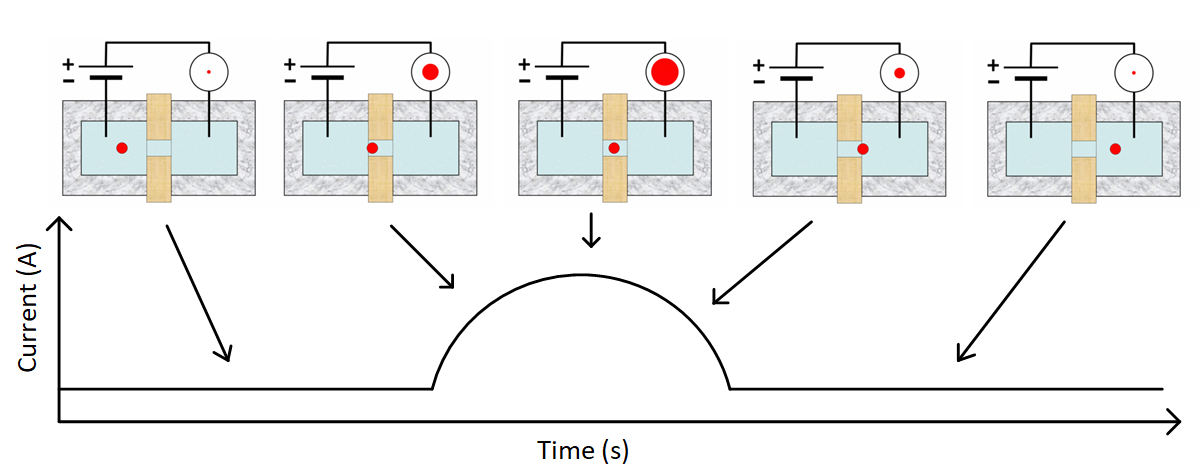
\includegraphics[width=1\textwidth]{CoulterCounter}
    \caption{Observed current response of a Coulter Counter for different particle position in the microchannel.}
    \label{fig:CoulterCounter}
\end{figure}

IFC can effectively be considered a generalization of the Coulter Counter since it measures not only the DC resistance, but the impedance value at any given frequency. When done as a spectroscopy, it leads to an adequate characterization of the dielectric properties of the cells flowing inside a microchannel, which can be used in association with their single-shell or double-shell models described in \autoref{sec:CellModel} to retrieve some important characteristics of single-celled organisms. \cite{Opitz2019, Cheung2010, Xu2016}. The complex permittivity of the mixture can be retrieved from the complex impedance knowing the geometrical parameters of the microchannel and electrodes \cite{Sun2010,Xu2016}. However, since the permittivity cannot physically be interacted with (hence it cannot be directly measure), the impedance of the mixture $Z_{mix}$ must first be acquired and converted to a permittivity using mathematical functions. As described before in \autoref{chap:Biosensors}, an impedance depends on geometrical and material factors. The complex impedance of the cell-medium system, $Z_{mix}$, can be approximated considering both the geometrical and material parameters \cite{Xu2016,morgan2006single}:
\begin{equation}
\label{eq:Zmixture}
Z_{mix}=\frac{1}{j \omega \varepsilon_{mix} l \kappa}
\end{equation}
The mathematics quickly becomes complicated here to convert from the mixture’s impedance to the mixture’s permittivity. This is the case since the volume factor $\phi$ between the cell and detection area is quite high, creating a fringing effect at the electrodes, as shown in \autoref{fig:FringingEffect}. This fringing effect could be considered inconsequential when the electric field is homogeneous and for low volume fraction cases, but that is rarely the case in IFC. Thus, the most challenging problem is how to calculate this fringing effect through the the cell constant $\kappa$, which influences both the volume fraction, and the impedance of the mixture. The Schwarz-Christoffel mapping \cite{Schwarz1869, Christoffel1867} needs to be used to calculate $\kappa$, which makes use of the complete elliptic integral of the first kind, of the complementary integral, and of the modulus of the elliptic function \cite{Xu2016,morgan2006single}. This mathematic being out of the scope of this memoir, only the mixture impedance $Z_{mix}$ will be measured in this study, and the cell parameters will be assumed retrieved. \par
\begin{figure}[h]
    \centering
    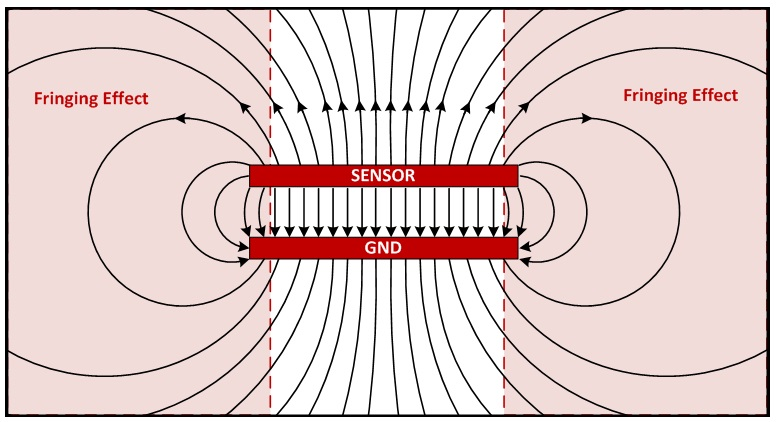
\includegraphics[width=0.8\textwidth]{FringingEffect}
    \caption{Fringing effect as modelized on parallel electrodes. \citep{FringingEffect}}
    \label{fig:FringingEffect}
\end{figure}

A simple alternative to the mathematics associated with the size determination of particles is given in \citep{De_Ninno2017,caselli2018novel}. An estimation of the particle diameter $D$ can be found with a fit to the cubic root of the measured impedance magnitude difference observed when a particle passes the electrode pairs in the channel:
\begin{equation}
\label{eq:sizeEstimation}
D = G (\lvert \Delta Z_{1} \rvert+ \lvert \Delta Z_{2} \rvert){^{1/3}}
\end{equation}
Where $G$ is a constant that accounts for a multitude of factors, including the electrode configurations, the magnitude and frequency of the excitation signal, the filter bandwidth, the channel depth and width, the electrode sizes, the EDL capacitance $C_{edl}$, the buffer conductivity, and the circuit gains. Ths constant $G$ can be determined empirically by testing the IFC system with circular beads of know diameters, then adjusting the coefficient $G$ until the diameters estimated using \autoref{eq:sizeEstimation} match the beads diameters \cite{caselli2018novel}. Such a size estimation is shown in \autoref{fig:Caselli2018DiameterEstimation}. \par
\begin{figure}[h]
    \centering
    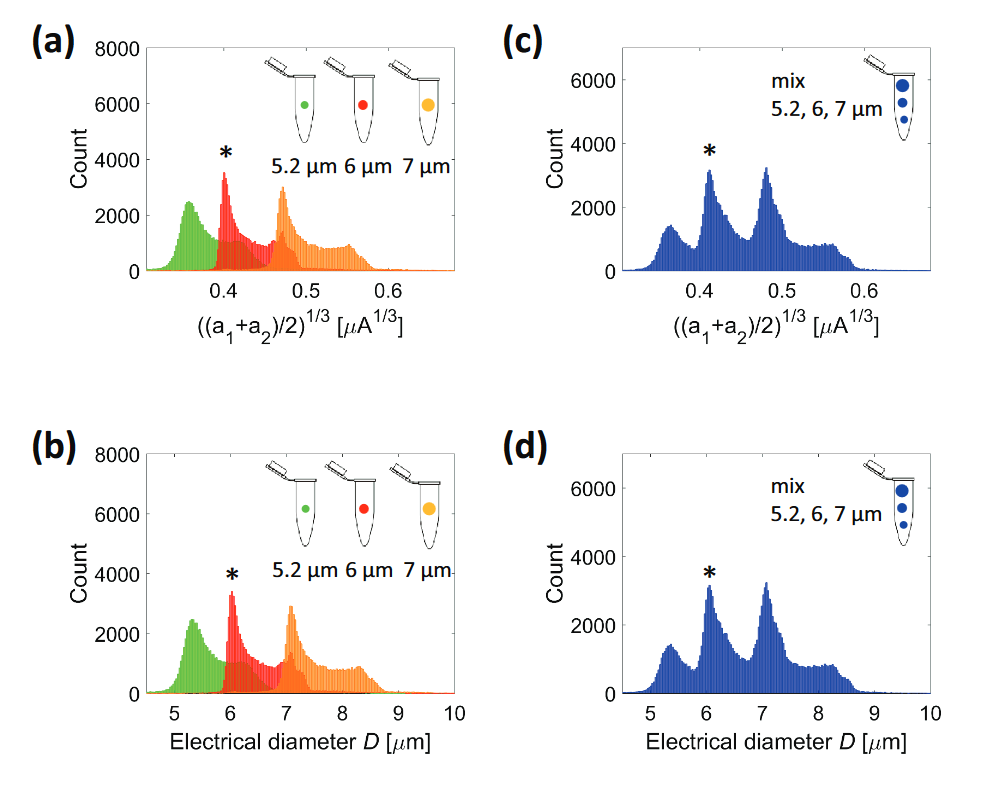
\includegraphics[width=0.8\textwidth]{Caselli2018DiameterEstimation}
    \caption{Electrical diameter $D$ estimation using equation \autoref{eq:sizeEstimation}. \citep{caselli2018novel}}
    \label{fig:Caselli2018DiameterEstimation}
\end{figure}

It is also possible to measure the particle velocity by dividing the distance between the electrode pairs $L$ with the time it took for the particle to go from one electrode to the other $\Delta t$ (which is the time difference between the two impedance maximums). Such a velocity $v$ is described as :
\begin{equation}
\label{eq:VelocityEstimation}
v = \frac{L}{\Delta t}
\end{equation}
Based on \autoref{eq:Zmixture}, \autoref{eq:sizeEstimation}, and those for whole-cell analysis presented in \autoref{sec:CellModel}, it is possible to find design parameters for the microfluidic channel and coplanar electrodes. From \autoref{eq:Zmixture}, only the volume fraction $\phi$ through the electrode width $w$, electrode length $l$, channel height $h$, and cell constant $\kappa$ (through the ratio of $w$ to $h$) can be influenced by design; the other parameters being function of the cell or medium. This means that a maximization of the volume fraction will create the maximum difference in impedance between the mixture and cell. This is intuitively correct since the cell would then replace the maximum quantity possible of mixture for the impedance measurement. Maximizing $\phi$ requires that the channel and electrodes be as small as possible. There are, however, technical limitations to the minimum size of both, which are described in \autoref{sec:FabricationMicrofluidics} and \autoref{sec:ElectrodeDesign}. To maximize the volume fraction, it is necessary to know beforehand the size of the largest particle to flow in the channel. This means that to obtain a sufficient precision for small particles, a small channel must be constructed, which will block the larger particles. This compromise means that the channel in IFC must be designed with the size of the particles in mind. The channel should be made so that the length and height of the microchannel are comparable \cite{Gawad2004}. Indeed, decreasing the length of the channel is associated with lower thermal noise. It however creates a non-uniform current density in the channel’s axis, which require further signal processing to correct the end effects \cite{Gawad2004}. A differential design is also of a prime importance in IFC to decrease the background noise and increase the sensitivity to the flowing particles \cite{Xu2016,horowitz1989art}. \par 

The electrodes size should be minimized until the impact of the substrate dielectric begins to short-circuit the frequency of interests, as a drop in precision is observed at that moment, as described in \autoref{sec:ElectrodeDesign}. Facing electrodes are a better choice for IFC than coplanar electrodes because the electrical field is uniform along the path of the particles, which greatly simplifies the mathematics associated with retrieving the cells properties from the impedance values \cite{Xu2016}. It also greatly reduces the fringing effect of the electrodes, which tends to complicate the measurement. Facing electrodes are, however, difficult to construct using lithography techniques. Coplanar electrodes being 2d structures, they can be made efficiently using a lithography mask or directly on a PCB \cite{Sun2010}. \par

These electrodes are generally fabricated with materials resistant to oxidation, such as gold or platinum. Those metals are used because of their convenience in casting for such small dimensions, for their unlimited lifetime, and since other types of electrodes such as Ag/AgCl are unsuitable for high excitation frequency \cite{Sun2010}. However, they hinder the charge exchange with the ionic solution, which causes a polarization of the ion-electrode surface, causing a double-layer capacitance $C_{dl}$ to form at the interface. The frequency must be increased beyond the EDL to access the solution resistance modulated by the presence of particles without being too affected by the EDL. For the case of gold/cell culture buffer, $C_{dl}$  is of about 0.1pF per $\mu m^2$ of electrode area \cite{Carminati2017}. One solution to reduce the EDL is to increase the electrode surface area. The throughput of IFC sensors can be improved using multiple microchannels in parallel or by increasing the number of electrodes per channels \cite{Sun2010}. \par

The frequency behaviors in IFC systems are shown in \autoref{fig:CellFrequency} and \autoref{fig:ElectrodeResponse}. For frequencies lower than 100kHz, the electrical double-layer dominates the measured impedance in micron scale electrodes, which reduces the detection sensibility of particles \cite{Xu2016,Gawad2004,Bouzid2022NEWCAS}. For intermediate frequencies (1-10MHz), the cell membrane becomes the main cause of impedance change. For higher frequencies than 10MHz, the membrane becomes effectively short-circuited, which makes the cytoplasm responsible for the variation in impedance. The impedimetric behavior of IFC sensors generally is stable from 100kHz to 10MHz. Above that, the PCB dielectric shunts the channel impedance, and the parasitics of the measurement electronics affect the results \cite{Gawad2004,Bouzid2022NEWCAS}. \par
\begin{figure}[h]
    \centering
    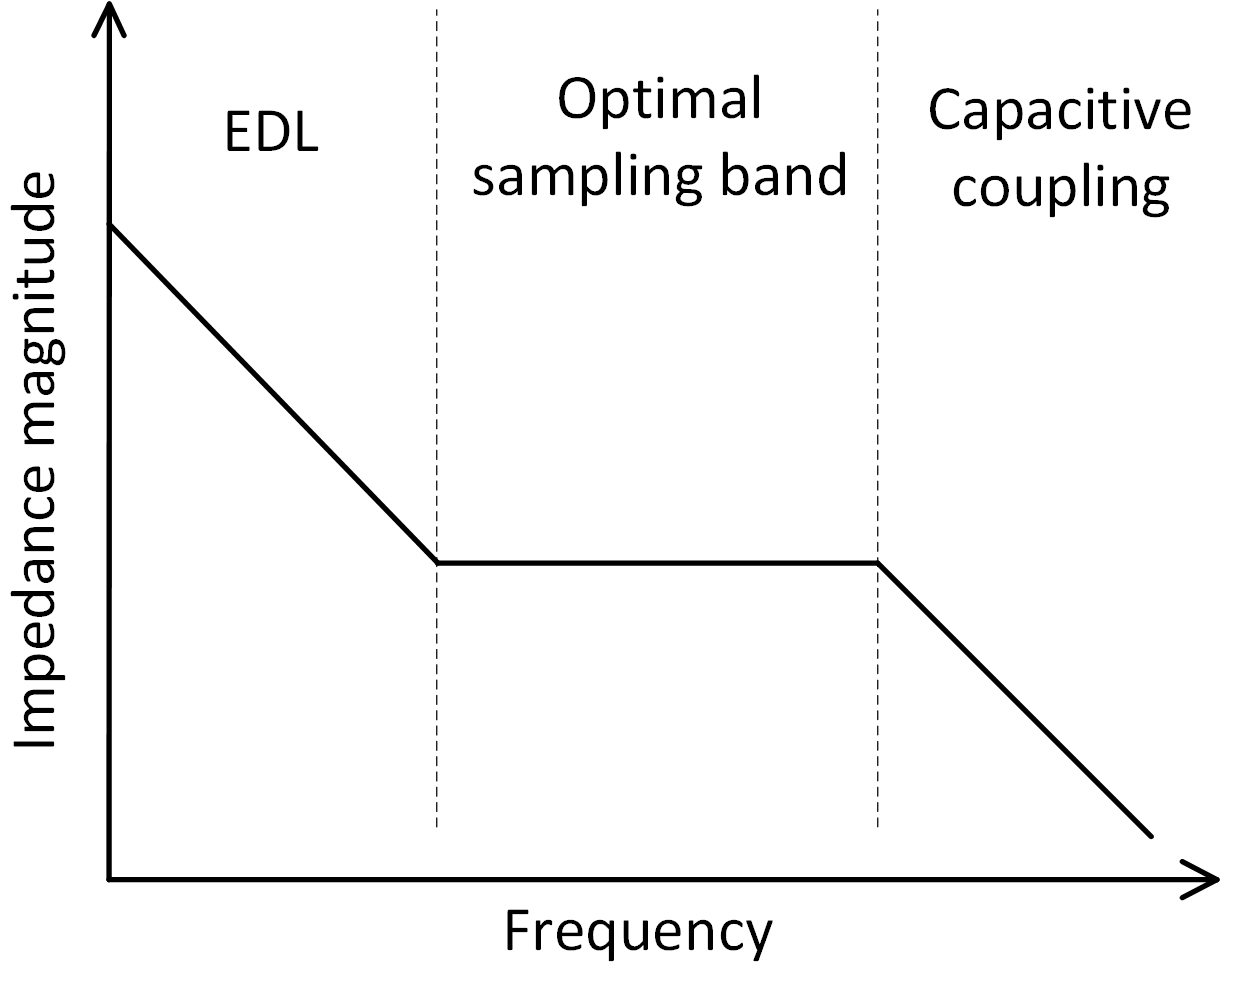
\includegraphics[width=0.6\textwidth]{ElectrodeResponse}
    \caption{Frequency behaviors observed in IFC. The optimal measurement zone is in-between the EDL and the high-frequency capacitive coupling. }
    \label{fig:ElectrodeResponse}
\end{figure}

The opacity, which is the ratio of a high frequency impedance to a low frequency impedance, is often used in particle scatter diagram in IFC. It acts as a unitless dimension for 2d-representation \cite{Xu2016}. Such type of representation can help visually differentiate or regress cell sizes and morphologies, as well as their condition or life phase. An example scattergram is shown in \autoref{fig:ScatterGram}. \par
\begin{figure}[h]
    \centering
    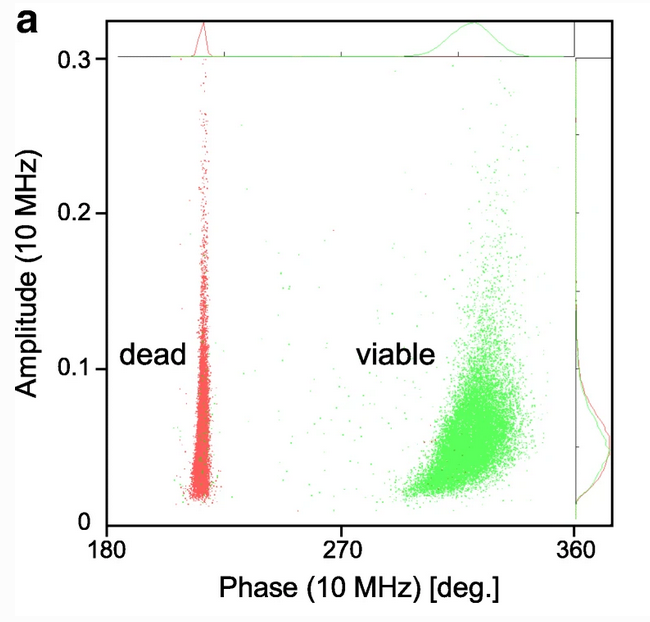
\includegraphics[width=0.6\textwidth]{ScatterGram}
    \caption{Impedance amplitude and phase scattergram used to differentiate between live and dead cells.\citep{Opitz2019}}
    \label{fig:ScatterGram}
\end{figure}

IFC has already proven its usefulness for cell differentiation (stained vs unstained, alive vs dead cells) \cite{Carminati2017,david2012viability, prakash2005cmos,Opitz2019}. The soft cell membrane of animal cells loses their electrical properties upon death, which translates into a decrease of the measured impedance difference at intermediate frequencies. Using such tricks, it is possible to differentiate different cells state or modification to their environment. These techniques are however not generalizable to every microparticles. A case-by-case methodology must be elaborated. For instance, bacteria and yeast generally have rigid cell walls, meaning that they keep their membrane properties upon death. Probing at higher frequency inside the cytoplasm could, however, solve this issue \cite{david2012viability,Opitz2019}. Information on the cell membrane capacitance, used in conjunction with the cell size, can be sufficient to discriminate between different blood leukocytes. Using high frequency measurements can determine if a cell is invaded by parasites by probing the cell’s internal composition \cite{Sun2010}.  IFC can also be used to gain information about the status of the cell culture. For example, there is a phase shift towards lower value of phase when the cell population transitions from the exponential to the stationary growth phase. In yeast culture, the cells begin to grow in the lag phase, before dividing and then maintaining a smaller average cell similar to that of a dead cell \cite{Opitz2019}. \par

The differential impedance spikes observed at the output are used to count the number of particles passing in the channel, as well as determining the particle size, morphology, and composition. A simple detection algorithm would be to fix a rigid threshold for a specific impedance value such that whenever the impedance goes above that threshold, a particle is recognized by the algorithm. The amplitude and size of that pattern can be used to deduce the cell parameters and fluid flow. Other more complex detection methods can be used, such as segmentation, autocorrelation, leveraging the odd symmetry of differential pulses, machine learning , etc. \cite{Carminati2017}. \par

The position of the cell in the channel influences the measured signal due to the non-homogeneous electrical field distribution of coplanar electrodes. A higher particle in the channel will experience weaker electrical field than a low particle, which will result in a lower perceived amplitude \cite{De_Ninno2017,caselli2018novel}. Since the amplitude of the spike is used to infer the cell properties, a significant error is thus observed. three solutions can be used to counter this problematic: (1) Using parallel facing electrodes placed diagonally opposed in the channel, as proposed by \citep{caselli2018novel}. This technique however requires parallel electrodes, which adds complexity to the microfabrication. (2) A The structure of the electrodes themselves can be modified, as shown in \autoref{fig:DeNinno2017}, to create specific signal pattern whose shape can be used to identify the vertical position of the particle in the channel (such shapes are also found to be more robust against noise)  \cite{Carminati2017,De_Ninno2017}. The relative prominence of the shapes obtained, coupled to the transit time of such shape, are parameters that depend on the geometry of the channel and electrodes, such that corrected particles parameters can be retrieved from post-processing calculations. This method, however, reduces the sensibility of the measured pulses since the sensing volume increases when using multiple electrodes \cite{petchakup2017advances}. (3) Centering techniques such as dielectrophoresis, acoustophoresis, inertial focusing and sheath flows can be used in the microfluidics to put the cells exactly where they are needed. This second solution is, however, more complicated and has quite a lot of shortcomings, but at least doesn’t require complex post-processing calculations \cite{De_Ninno2017}. \par
\begin{figure}[h]
    \centering
    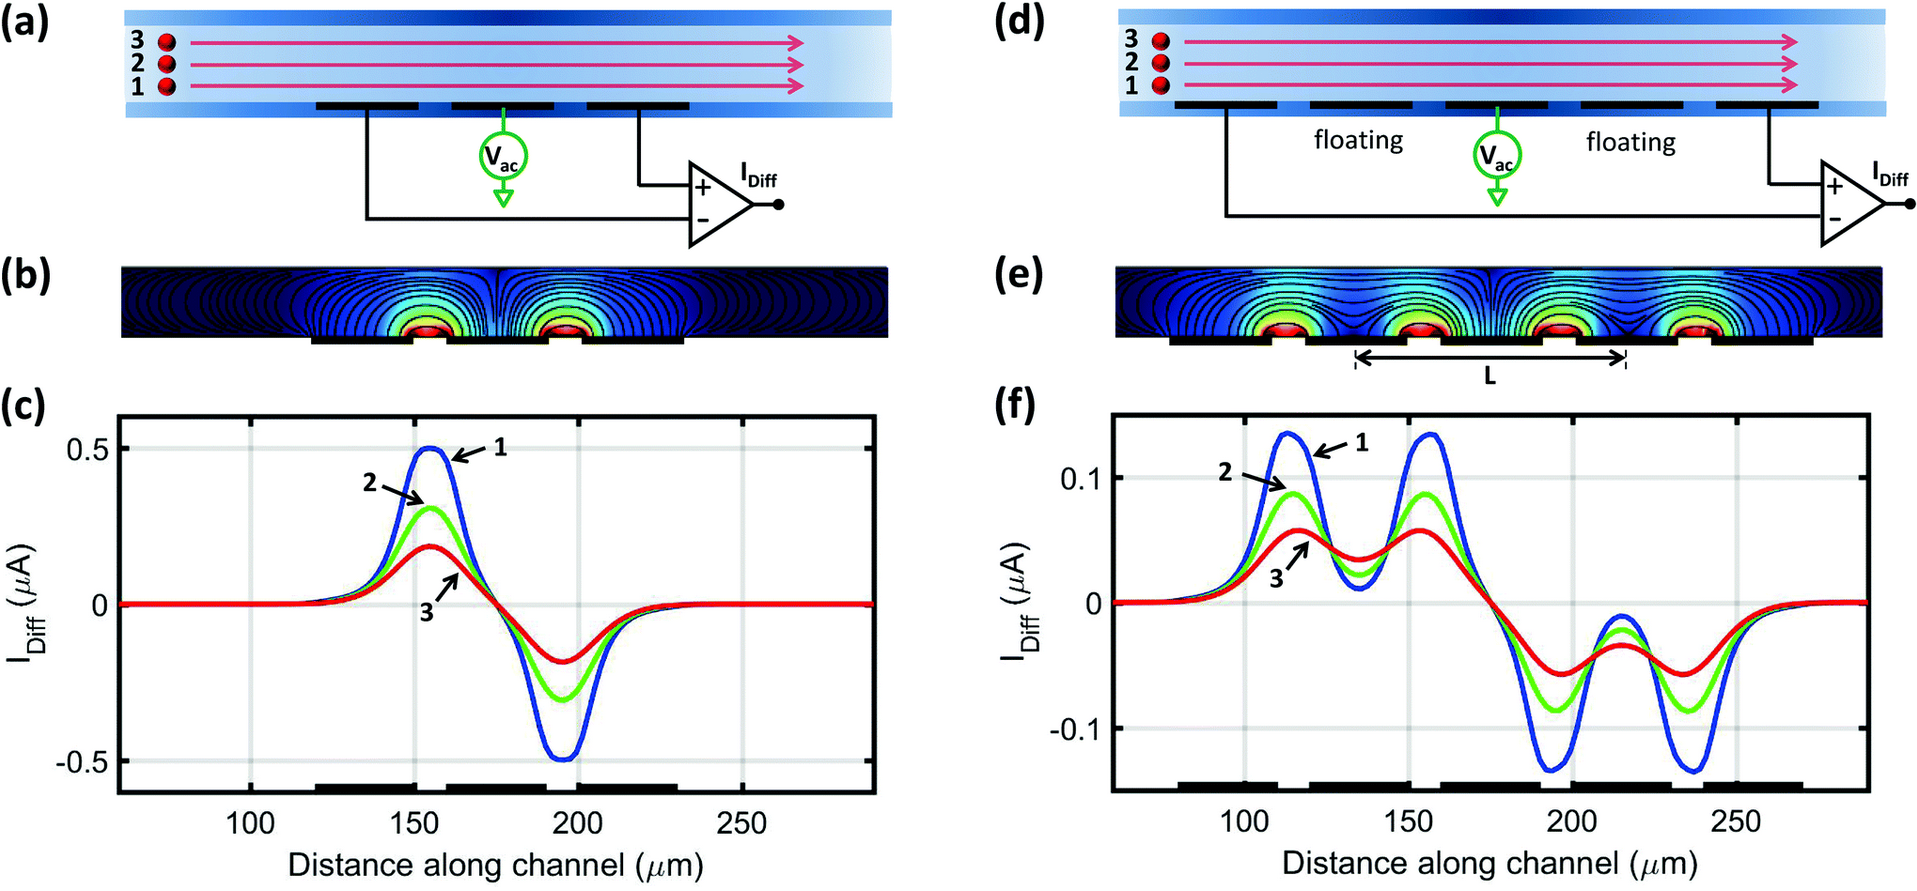
\includegraphics[width=1\textwidth]{images/DeNinno2017.png}
    \caption{A conventional differential 3-coplanar electrodes signal response, compared to the configuration when two floating electrodes are added. Note the difference in signal response in function of the height of the particle in the channel.\citep{De_Ninno2017}}
    \label{fig:DeNinno2017}
\end{figure}

IFC is quite tolerant to multiple medium conductivity and conditions. A conductivity between 2 and 10 mS/cm is generally deemed adequate. The number of cells should however be kept low enough such that the channel does not clog or that multiple particles pass the electrodes at the same time, resulting in a bigger signal output. Simply diluting the sample is an effective action to counter that. Adding a surfactant to the buffer, such as soap, proves itself adequate to prevent chain forming microparticles. A filter might also be used to remove large impurities \cite{Opitz2019}. These fluidics concerns will be discussed in \autoref{chap:Microfluidics}.